%%%%%%%%%%%%%%%
%
% Modelo de Teses NÃO OFICAL
%
%%%%%%%%%%%%%%%



\documentclass[11pt,twoside]{estiloUBI}


%%%%%%%%%%%%%%%%%%%%%%%%%%%%%%%%%%%%%%%%%%%%%%%%%%%%%%%%%%%%%%%%%%%%%%%%%%%%%%%%%%%%%%%%%%%%%%%%%%%%%%%%%%%%%%
%% Este é o ficheiro formatacaoUBI.tex - NÃO EDITAR excepto a secção hypersetup!
%% Define a formatação a ser usada em teses apresentadadas na Universidade da Beira Interior, seguindo o despacho Reitoral nº 49/R/2010. Revogado pelo despacho Reitoral nº 2019/R/630
%% Versão 3.0 - 2020/01/31 - Adaptado às normas do despacho Reitoral nº 2019/R/630
%% Versão 2.2 - 01/06/2016 - Podem aparecer as palavras "Figura" e "Tabela" nas respectivas listas
%% Versão 2.1 - 28/03/2014 - Agora compila com o XeLaTeX por causa do tipo de fonte, incluido o estilo de biblipgrafia IEEE, possibilidade de escolha de tipo de fonte matemático
%% Versão 2.0 - 10/11/2011 - Bibliografia agora aparece no índice
%% Versão 1.9 - 10/10/2011 - Resolvido problema em que o texto nas tabelas aparecia em cima da linha superior
%% Versão 1.8 - 12/07/2011 - Legendas são agora centradas
%% Versão 1.7 - 8/07/2011 - Correcção de algumas medidas de acordo com novo modelo de Word
%% Versão 1.6 - 1/07/2011 - Trebuchet inserido como fonte principal
%% Adaptado do original de Oliver Commowick para estar de acordo com as regras do Despacho nº 49/R/2010
%% Adaptação por João Ferro, Norberto Barroca, Luís Borges, Rui Paulo, Aleksandra Nadziejko - Instituto de Telecomunicações - DEM/UBI, Paulo Machado - Departamento de Ciências Aeroespaciais/UBI.
%% 
%% Agradecimento especial a Stefan_K da latex-community.org pela ajuda com os códigos de tabela e equação.
%% A versão actual pode ser alterada sem aviso prévio.
%% Download da última versão em área reservada: http://www.UBI.pt
%% Uso e distribuição de acordo com a licenca GNU GPL.
%% 
%%    Este programa é um software livre: você pode redistribui-lo e/ou 
%%
%%		modificá-lo dentro dos termos da Licença Pública Geral GNU como 
%%
%%		publicada pela Free Software Foundation, na versão 3 da 
%%
%%		Licença, ou (na sua opinião) qualquer versão.
%%
%%
%%
%%		Este programa é distribuido na esperança que possa ser útil, 
%%
%%		mas SEM NENHUMA GARANTIA; sem uma garantia implícita de ADEQUAÇÃO a qualquer
%%
%%		MERCADO ou APLICAÇÃO EM PARTICULAR. Veja a
%%
%%		Licença Pública Geral GNU para maiores detalhes.
%%
%%
%%
%%		Você deve ter recebido uma cópia da Licença Pública Geral GNU
%%
%%		junto com este programa, se não, veja <http://www.gnu.org/licenses/>.
%%%%%%%%%%%%%%%%%%%%%%%%%%%%%%%%%%%%%%%%%%%%%%%%%%%%%%%%%%%%%%%%%%%%%%%%%%%%%%%%%%%%%%%%%%%%%%%%%%%%%%%%%%%%%%


% Pacotes a incluir
\usepackage{mathspec}
\usepackage{fontspec}
\usepackage{amsmath,amscd,amsthm,xspace}	%Pacotes matemáticos 
\usepackage{amssymb}						%Fontes extra para matemáticos   http://www.ctan.org/tex-archive/fonts/amsfonts
%\usepackage[math]{kurier} %descomentar para colocar tipo de letra aproximado ao Trebuchet nos ambientes matemáticos

%\usepackage[latin1]{inputenc}		%este faz falta na versão normal, mas em XeLaTeX tem que ser comentado		%Permitir caracteres acentuados  http://www.ctan.org/pkg/inputenc
%\usepackage[T1]{fontenc}					%este faz falta na versão normal, mas em XeLaTeX tem que ser comentado		%Permitir caracteresespeciais  http://www.ctan.org/pkg/fontenc

\usepackage[a4paper,left=3cm,right=2.5cm,top=2.5cm,bottom=2.5cm]{geometry}	%Papel A4, com margens
%\renewcommand{\baselinestretch}{1.05}

\usepackage{aecompl}								%Permitir fontes vituais para codificação T1  http://www.ctan.org/tex-archive/fonts/ae
\usepackage[center,nooneline,font={footnotesize}]{caption}			%Legenda: centrada, tamanho de nota rodapé  http://www.ctan.org/pkg/caption
\setlength{\parindent}{0.53cm}							%Sem tabulação em cada novo parágrafo
%\usepackage{parskip}								%Layout with zero \parindent, non-zero \parskip http://www.ctan.org/pkg/parskip
%\setlength{\parskip}{0.53cm}



%% O código seguinte permite gerar um mini indice de capitulo (não referido no despacho reitoral)
% \usepackage[nottoc, notlof, notlot]{tocbibind}
% \usepackage{minitoc}
% \setcounter{minitocdepth}{2}
% \mtcindent=15pt
%%Usar \minitoc para colocar o mini indice de capitulo


%% Verificar se saída é pdf directo e ajustar o formato imagens a isso
%\usepackage{ifpdf}
%\ifpdf
%  \usepackage[pdftex]{graphicx}							%Inserir gráficos  http://ctan.org/pkg/graphicx
\usepackage{graphicx}
%    \DeclareGraphicsExtensions{.jpg,.png} 					%Pdf directo apenas compativel com jpg, png...
  \usepackage[pagebackref,hyperindex=true]{hyperref}				%O pacote hyperref é usada para lidar com comandos referência cruzada  http://ctan.org/pkg/hyperref
%\else
%  \usepackage{graphicx}
%  \DeclareGraphicsExtensions{.ps,.eps}						%DVI directo apenas compativel com ps, eps...
%  \usepackage[dvipdfm,pagebackref,hyperindex=true]{hyperref}
%\fi


\graphicspath{{.}{imagens/}}							%Directorio das imagens


%%Links do pdf
\usepackage{color}								%Pacote de gestão de cor
\definecolor{linkcol}{rgb}{0,0,0} 						%Cor das hiperligações (preto)
\definecolor{citecol}{rgb}{0,0,0} 						%Cor das referências à bibliografia no texto (preto)


%% O código seguinte será incluído no pdf gerado http://www.tug.org/applications/hyperref/manual.html
%%Visto nas propriedades do documento
% \hypersetup
% {
% bookmarksopen=true,
% pdftitle="Tese",		%Título
% pdfauthor="João", 		%Autor
% pdfsubject="Tese", 		%Assunto
% pdfmenubar=true,		%Mostrar barra menus
% pdfhighlight=/O, 		%Efeito ao clicar link
% colorlinks=true, 		%Cor em hiperligações
% pdfpagemode=UseNone, 		%Nenhum modo de páginas
% pdfpagelayout=SinglePage, 	%Abertura em modo de página simples
% pdffitwindow=true, 		%Adaptar página à janela
% linkcolor=linkcol, 		%Cor das ligações internas do documento
% citecolor=citecol, 		%Cor das referências à bibliografia no texto
% urlcolor=linkcol 		%Cor das hiperligações
% }


%%Definições variadas
\setcounter{secnumdepth}{3}
\setcounter{tocdepth}{2}


%%Comandos e atalhos para algumas funções matemáticas
\newcommand{\pd}[2]{\frac{\partial #1}{\partial #2}}
\def\abs{\operatorname{abs}}
\def\argmax{\operatornamewithlimits{arg\,max}}
\def\argmin{\operatornamewithlimits{arg\,min}}
\def\diag{\operatorname{Diag}}
\newcommand{\eqRef}[1]{(\ref{#1})}


%%Para rotação de figuras e tabelas http://www.ctan.org/tex-archive/macros/latex/contrib/rotating
 \usepackage{rotating}
  
	
%%Cabeçalho e rodapé http://www.ctan.org/tex-archive/macros/latex/contrib/fancyhdr
\usepackage{fancyhdr}                   						%Fancy Header and Footer
\pagestyle{fancy}                      							%Cabeçalho e rodapé estilo fancy
\fancyfoot{}                            						%Apaga rodapé actual
\fancyhead{}										%Apaga cabeçalho actual
\fancyfoot[CE,CO]{\thepage}   								%Número de paginas no exterior C=cener, L=left, E=even, R=right, O=Odd
\newcommand{\cabecalho}[1]{\fancyhead[RE,LO]{\bfseries{#1}}}				%Nome da tese no cabeçalho
\let\headruleORIG\headrule
\renewcommand{\headrule}{\color{black} \headruleORIG}
\renewcommand{\headrulewidth}{0pt}							%Régua para cabecalho, 0pt=off, 1pt=on


%Formatação dos tipos de letra
\newcommand{\capitulos}{\fontsize{18pt}{11pt}\bfseries\selectfont}%Capítulo: 18pt, negrito
\newcommand{\titulos}{\fontsize{18pt}{11pt}\bfseries\selectfont}	%Titulos: 18pt, negrito
\newcommand{\seccao}{\fontsize{14pt}{20pt}\bfseries\selectfont}	%Secção: 14pt, negrito
\newcommand{\subseccao}{\fontsize{12pt}{14pt}\selectfont}			%subsecção: 12pt, normal
\renewcommand{\footnotesize}{\fontsize{9pt}{12pt}\selectfont}		%Nota rodapé: 9pt, espacamento 1 linha
\renewcommand{\Huge}{\titulos}


%Folha de rosto
\newcommand{\rostoubi}{\fontsize{14pt}{14pt}\selectfont}	 %Texto a dizer UBI 14pt, normal
\newcommand{\rostotitulo}{\fontsize{18pt}{18pt}\selectfont}%Titulo da tese: 18pt, (+negrito)
\newcommand{\rostosubtit}{\fontsize{16pt}{16pt}\selectfont}%Titulo da tese: 16pt, (+negrito)
\newcommand{\rostonomes}{\fontsize{14pt}{14pt}\selectfont}	 %Nome autor, curso: 14pt, (+negrito)
\newcommand{\rostooutros}{\fontsize{12pt}{12pt}\selectfont}%Local e data: 12pt, (+negrito)
\newcommand{\rostofac}{\fontsize{12.5pt}{12.5pt}\selectfont}	%Faculdade: 12.5pt




%%Passar para português
%\newcommand{\portugues}{\usepackage[portuguese]{babel}		%Descomentar para escrever com regras em Português sem ser em XeLaTeX  http://www.ctan.org/pkg/babel  								% Users of X∃TeX are ad­vised to use poly­glos­sia rather than Ba­bel.

\newcommand{\portugues}{\usepackage{polyglossia} %Comentar para escrever sem ser em modo XeLaTeX http://www.ctan.org/tex-archive/macros/latex/contrib/polyglossia
\setmainlanguage{portuges}                       %Comentar para escrever sem ser em modo XeLaTeX

\addto\captionsportuguese{\renewcommand{\contentsname}{Índice}}
\addto\captionsportuguese{\renewcommand{\indexname}{Índice Remissivo}}}

%linhas das tabelas e afins
\usepackage{colortbl}									%Adicionar cor às tabelas  http://www.ctan.org/tex-archive/macros/latex/contrib/colortbl/
\arrayrulecolor{black}									%Preto


%Estilo plain modificado
\fancypagestyle{plain}{
  %\fancyhead{}	
  %\fancyfoot{}
  \renewcommand{\headrulewidth}{0pt}
}


%%Para algoritmos  http://www.ctan.org/tex-archive/macros/latex/contrib/algorithms/
\usepackage{algorithm}
\usepackage[noend]{algorithmic}


%%Páginas em branco geradas antes de capítulos têm de vir numeradas
\makeatletter

\def\cleardoublepage{\clearpage\if@twoside \ifodd\c@page\else%
  \hbox{}%
  \thispagestyle{plain}%              							%Páginas em branco usam estilo plain
  \newpage%
  \if@twocolumn\hbox{}\newpage\fi\fi\fi}

\makeatother


%%Tabela com 9pt
%\makeatletter										%O código comentado apresentado apresenta problemas
%\renewenvironment{table}{%								%Procurar no forum http://latex-community.org, tópico "Equation Numbering and Table Font Size''
  %\@float{table}\footnotesize}
  %{\end@float}
%\makeatother
\usepackage{etoolbox}									%Para modificar o tamanho de letra na tabela http://ctan.org/pkg/etoolbox
\AtBeginEnvironment{tabular}{\footnotesize}						%Procurar no forum http://latex-community.org, tópico "Equation Numbering and Table Font Size''


%%Número de equação centrado com equação
\makeatletter										%Explicação  http://tex.stackexchange.com/questions/8351/what-do-makeatletter-and-makeatother-do
\def\place@tag{\quad\boxz@}								%Comentar esta linha para alinhar número da equação à direita
\makeatother
\let\equation\align
\let\endequation\endalign
 

%%Código herdado
\newenvironment{maxime}[1]
{
\vspace*{0cm}
\hfill
\begin{minipage}{0.5\textwidth}%
%\rule[0.5ex]{\textwidth}{0.1mm}\\%
\hrulefill $\:$ {\bf #1}\\
%\vspace*{-0.25cm}
\it 
}%
{%

\hrulefill
\vspace*{0.5cm}%
\end{minipage}
}

%mninitoc
%\let\minitocORIG\minitoc
%\renewcommand{\minitoc}{\minitocORIG \vspace{1.5em}}

\usepackage{multirow}					%Create tab­u­lar cells http://www.ctan.org/tex-archive/macros/latex/contrib/multirow
% \usepackage{slashbox}					%Pro­duce tab­u­lar cells with di­ag­o­nal lines in them http://www.ctan.org/pkg/slashbox

\newenvironment{bulletList}				%http://en.wikibooks.org/wiki/LaTeX/List_Structures
{ \begin{list}%
	{$\bullet$}%
	{\setlength{\labelwidth}{25pt}%
	 \setlength{\leftmargin}{30pt}%
	 \setlength{\itemsep}{\parsep}}}%
{ \end{list} }

\newtheorem{definition}{Définition}
\renewcommand{\epsilon}{\varepsilon}

% centered page environment

\newenvironment{vcenterpage}
%{\newpage\vspace*{\fill}\fancyhf{}\renewcommand{\headrulewidth}{0pt}}
{\newpage\vspace*{\fill}\renewcommand{\headrulewidth}{0pt}}
{\vspace*{\fill}\par\pagebreak}

\usepackage{setspace}					%Pro­vides sup­port for set­ting the spac­ing be­tween lines http://www.ctan.org/tex-archive/macros/latex/contrib/setspace
\usepackage{tabularx}					%The pack­age de­fines an en­vi­ron­ment tab­u­larx, an ex­ten­sion of tab­u­lar  http://www.ctan.org/pkg/tabularx
\usepackage{makeidx}					%Index processor  http://www.ctan.org/tex-archive/indexing/makeindex
\newcolumntype{Y}{>{\raggedright\arraybackslash}X}

%% Inicio do bloco
%% Descomentando o este bloco de comandos as  palavras "Figura" e "Tabelas" vão aparecer por extenso nas respectivas Listas
%%
%% Comentado aparece:
%%Lista de Figuras
%%		2.1 Circuito básico com uma fonte de tensão contínua (V) e uma resistência atraves-
%%			sada por uma corrente I. . . . . . . . . . . . . . . . . . . . . . . . . . . . . .3
%%
%% Descomentando aparece
%% 		Figura 2.1 Circuito básico com uma fonte de tensão contínua (V) e uma resistência
%%      atravessada por uma corrente I. . . . . . . . . . . . . . . . . . . . . .3
%%
%\usepackage[titles]{tocloft}
%\newlength{\mylen}
%
%\renewcommand{\cftfigpresnum}{\figurename\enspace}
%\renewcommand{\cftfigaftersnum}{ }
%\settowidth{\mylen}{\cftfigpresnum\cftfigaftersnum}
%\addtolength{\cftfignumwidth}{\mylen}
%
%\renewcommand{\cfttabpresnum}{\tablename\enspace}
%\renewcommand{\cfttabaftersnum}{ }
%\settowidth{\mylen}{\cfttabpresnum\cfttabaftersnum}
%\addtolength{\cfttabnumwidth}{\mylen}
%% Fim do Bloco



\usepackage{fontspec}
\usepackage{comment}
\setmainfont{Georgia}
\usepackage{hyphenat}
\usepackage{listings}
\usepackage{pgfgantt}
\hyphenation{he-lio-trope opos-sum}

\usepackage{svg}
%%Comentar a linha seguinte se escrever a tese em inglês
%\portugues


%%Para índice remissivo
\makeindex


%%Escolher tipo de letra a usar:
%\usepackage{lmodern}												%Latin modern
%\usepackage{palatino}												%Palatino
%\usepackage{times}												    %Times


%%O comando seguinte insere o nome da tese no cabeçalho das páginas (comentar se não for pretendido)
%%\cabecalho{Inserir título da tese aqui (opcional)}



\begin{document}


%%O comando seguinte insere o espaçamento de 1.5 linhas
\onehalfspacing

%%Página de rosto
\pagenumbering{roman}
\begin{titlepage}
\begin{center}

\begin{flushright}
 
\includegraphics[height=3cm]{logo_ubi_vprincipal}\\
%\rostoubi UNIVERSIDADE DA BEIRA INTERIOR\\
%\rostofac Engenharia\\


\vspace{7.6cm}

\rostotitulo \textbf{Place holder} \\
\rostosubtit \textbf{Place holder 2}\\

\vspace{1.8cm}

\rostonomes \textbf{Carlos Francisco Caramelo Pinto}\\

\vspace{1.4cm}


% Escolher consoante seja Projeto de ESTÁGIO ou de DISSERTAÇÃO:
\rostooutros Master's dissertation planning
% No 2º semestre escolher consoante seja RELATÓRIO DE ESTÁGIO ou DISSERTAÇÃO:
%\rostooutros [] para obtenção do Grau de Mestre em\\

\rostonomes \textbf{Computer Science and Engineering}\\
\rostooutros (2nd degree cycle)\\

\vspace{3.3cm}

\rostooutros Supervisor: André Passos\\
\rostooutros Supervisor: Prof. Doctor Simão Melo de Sousa\\

\vspace{1.4cm}

\rostooutros \textbf{January 2024}

\end{flushright}

\end{center}
\end{titlepage}


%\dominitoc


%%Numeração das páginas
\pagestyle{fancy}


%%O comando a seguir gera uma página após a de rosto com cabeçalho e rodapé
\cleardoublepage

%%O comando a seguir permite que as costas da página de rosto não inclua cabeçalho mas rodapé (escolher entre este e outro)
%\newpage\mbox{}\thispagestyle{plain}\fancyhead{}


%%Dedicatória
%\newpage 
%\section*{\titulos{Dedicatória}}
%\vspace{0.5cm}
%Inserir dedicatória (opcional)
%\cleardoublepage
%\newpage 	
%\mbox{}
%\vfil
%\begin{center}
%Dedicated to...
%\end{center}
%\vfil
%\eject
%\cleardoublepage


%%Agradecimentos 
%\newpage 	
%\section*{\titulos{Agradecimentos}}
%\vspace{0.5cm}
%Agradecer a quem de direito (opcional)
%\cleardoublepage


%%Prefácio 
%\newpage 	
%\section*{\titulos{Prefácio}}
%\vspace{0.5cm}
%Opcional
%\cleardoublepage


%%Resumo+palavras-chave
%\newpage 	
%\section*{\titulos{Resumo}}
%\vspace{0.5cm}
%Resumo do trabalho
 
%\vspace{2.2cm}
%{\titulos{Palavras-chave}}
%
%\vspace{0.8cm}
%Inserir palavras-chave
%\cleardoublepage


%%Resumo alargado 
%\newpage 	
%\section*{\titulos{Resumo alargado}}
%\vspace{0.5cm}
%Unicamente para teses em língua estrangeira
%\cleardoublepage


%%abstract+keywords
%\newpage 	
%\section*{\titulos{Abstract}}
%\vspace{0.5cm}
%Abstract in English
%
%\vspace{2.2cm}
%{\titulos{Keywords}}
% 
%\vspace{0.8cm}
%Keywords in English
%\cleardoublepage


%%Índice
\tableofcontents





%%Lista de figuras
\listoffigures
\cleardoublepage	
%
%
%%%Lista de tabelas
%\listoftables
%\cleardoublepage


%%Abreviaturas
\newpage
\section*{\titulos{Acronymms}}
\vspace{0.5cm}
  \begin{tabularx}{\linewidth}{c p{0.5cm} Y}
    eBPF & & Extended Berkeley Packet Filter\cr 
    BPF & & Berkeley Packet Filter\cr
    JIT & & Just In Time\cr 
    CO-RE & & Compile Once - Run Everywhere\cr 
    BTF & & BPF Type Format\cr 
    LSM & & Linux Security Module\cr
    TOCTOU & & Time of Check to Time of Use\cr 
  \end{tabularx}
 \cleardoublepage
  

%% Os capitulos são inseridos a partir daqui 
 
\mainmatter

\chapter{Introduction}
\label{chap:int}


\section{Introduction}

%%%%% Probably talk here about the necessity of preventing data exfiltration in modern companies,. Why the need for security is massive, and the use of eBPF makes sense here.
Data exfiltration is the theft or unauthorized transfer of data from a device or network. This can occur in several ways, and the target data can vary from user credentials, intellectual property and company secrets.
The most common definition of data exfiltration is the unauthorized removal or movement of any data from a device.

The need for the prevention of data exfiltration is particularly pertinent in corporate settings, as there is the potential for the massive loss of revenue by companies which fall victim to these attacks. 
%we have a company which distributes machines to their paying costumers, and those machines are running a particular piece of software that is meant to be proprietary. There is the potential for costumers, through processes of reverse engineering, to try to replicate that piece of software. That presents a potential threat to the business model of said company, since what they are selling is not the software itself, but the machine, and we must also assume that there is a contractual obligation of the costumer to not try to reverse engineer said piece of software.

Extended Berkeley Packet Filter (eBPF) presents itself as the right tool to avoid these kind of attacks, since it is a technology that allows for the programming of the Linux kernel for networking, observability, tracing and security. It can effectively monitor the entirety of the system, as it runs inside the kernel, and detect and prevent any data exfiltration attempts.

\section{Motivation}

The main objective of this thesis is the development of an eBPF application that prevents data exfiltration from a given machine. This application will then go through a formal verification process. 

The fact that we use eBPF is particularly useful, since the classical approach of static configurations, although robust when configured statically during the provisioning of the machine, become brittle when deployed across a fleet of machines and in the face of changing policies. 

This application will serve the purpose of restricting services and capabilities inside the kernel, based on a per user or service approach, effectively armoring the system from unwanted accesses, either to services or files, thus preventing data exfiltration from said machine. 

It presents itself as quite a pertinent problem, both from and academic and business position, since the current approaches to tackle this problem are quite limited.
%eBPF programs are event-driven and are run when the kerne
%eBPF is the right tool for the job in this case, since currently it presents itself as a great monitoring tool. Being that eBPF runs inside the kernel, it has the ability to monitor all of the system calls made on that machine, and therefore detect, and potentially stop those data exfiltration attempts.
%%% Complete this with more information

\section{Document Organization}

This document is organized as follows:
\begin{enumerate}
    \item \textbf{Core Concepts and State of the Art} - This chapter aims to provide an overview of the Core Concepts necessary to understand the inner workings of eBPF, as well as the Linux kernel.
    \item \textbf{Problem Statement} - In this chapter we will describe the problem we are solving and a proposed solution to solve it. In it we will also elaborate on an experiment done to further sustain that the solution is a feasible one and, to finish the chapter, the tasks for the continuation of the development of this dissertation will be uncovered.
    \item \textbf{Conclusion} - This chapter serves the purpose of providing an overall conclusion to the document and the topics to be approached during this work.
\end{enumerate}

This is the organization of the document, where firstly we describe how this tool works, and then elaborating on the problem and solution that will be worked on in this dissertation.

\chapter{Core Concepts and State of the Art}

\section{Introduction}

In order to fully understand the inner workings of the eBPF tool and its potential for security and monitoring purposes in data exfiltration scenarios it is important to have a solid understanding of the core concepts of the Linux Kernel and eBPF, as well as the current state of the art in security and monitoring tools.
This chapter aims to provide an overview of both of these key topics.

\section{eBPF}

%% Discuss eBPF origins, the changes in recent years in the networking scene, and how LSM BPF makes eBPF a solid and reliable tool for security needs
eBPF is a revolutionary kernel technology that allows developers to write custom code that can be loaded into the kernel dynamically, changing the way the kernel behaves. This enables a new generation of highly performant networking, observability, and security tools.

This tool has its roots in the BSD Packet Filter, which are programs that are written in the BPF instruction set, deciding wheter to accept or reject a network packet. BPF came to stand for Berkeley Packet Filter, being first introduced to Linux in 1997.

BPF evolved to what eBPF, or extended BPF, in 2014, having several significant changes, such as:
\begin{enumerate}
    \item The BPF instruction set was overhauled to be more efficient on 64-bit machines, and the interpreter was entirely rewritten.
    \item eBPF \textit{maps} were introduced, which are data structures that can be accessed by BPF programs and by user space applications, allowing for the sharing of information between user space applications and BPF programs.
    \item The \texttt{bpf()} system call was added so that user space programs can interact with eBPF programs in the kernel.
    \item Several BPF helper functions were added
    \item The eBPF verifier was added to ensure that eBPF programs are safe to run.
\end{enumerate}

One of the biggest advancements in the eBPf toolset was made in 2020, when LSM PBF, was introduced, allowing for the attachment of eBPF programs as LSM, (Linux Security Module) kernel interface. This indicated a major use case for eBPF, bringing to light the fact that eBPF is a great platform for security tooling, in addition to networking and observability.

\subsection{Linux Kernel}
The Linux Kernel is the core component of the Linux operating system. It acts as a "bridge" between the hardware and the software layers, it communicates between the two, managing resources as efficiently as possible. 

The jobs of the Linux kernel are:
\begin{enumerate}
    \item \textbf{Process management}
        The kernel determines which processes can use the CPU, and for how long.
    \item \textbf{Memory Management}
        The kernel keeps track of how much memory is used to store what, and where.
    \item \textbf{Device drivers}
        The kernel acts as a mediator between the hardware and the processes.
    \item \textbf{System calls and Security}
        The kernel receives requests for service from processes.
\end{enumerate}


The kernel is quite complex, with around 30 million lines of code, meaning that if we were to try to make any changes to it, that would present a challenging task as making any change to a codebase requires some familiarity with it. Additionally, if the change made locally was to be made part of an official Linux release, it would not simply be a matter of writing code that works, it would have to be accepted by the community as a change that would benefit Linux as a whole, taking into account that Linux is a general purpose operating system. Assuming that the change was to be accepted, the waiting period until it would be accessible to everyone's machine would probably several years old, seeing that most users don't use the Linux kernel directly, but Linux distributions that might be using versions of the kernel that are several years old.

eBPF presents a quite ingenious solution to the problems mentioned above, seeing that eBPF programming does not mean direct interaction with kernel programming, and eBPf programs can be dynamically loaded and removed from the kernel. The latter presents one the great strengths of eBPF, as it instantly gets visibility over everything happening on the machine.

\subsection{System calls}

Applications run in an unprivileged layer called \textit{user space}, which can't access hardware directly. These applications make requests using the system call interface, requesting the kernel to act on its behalf. Since we're more used to the high level abstraction that modern programming languages, we can see an example of just how many system calls are made using the \texttt{strace} utility. For example, using the \texttt{ls} command involves 148 system calls.
%Insert screenshot of strace -c ls
Because applications are so heavily reliant on the kernel, it means we can learn a lot by observing its interactions with the kernel. With eBPF we can add instrumentation into the kernel to get these insights, and potentially prevent system calls from being executed.
Assuming we have a user who runs the \texttt{ls} command in a certain directory, eBPF tooling is able to intercept one of the several system calls involved in that command and prevent said command from being run. This makes it quite useful for security purposes, effectively modifying the kernel, running custom code whenever that system call is invoked.


\section{Formal Verification}


\begin{comment}
    
\chapter{Problem Statement, Experiments and Work Plan}

\section{Introduction}
The Problem Statement, Proposed Solution, Experiments, and Work Plan chapter is a crucial component of the thesis as it outlines the research problem, a possible solution to it, an experiment to further sustain that solution, and the plan for executing the research. In this chapter, we aim to present a clear and concise description of the problem we are solving, why it is important, and why the proposed solution is a valid one. The chapter will also include a detailed description of the experiments that will be conducted to validate the solution, as well as the work plan that outlines the tasks and the timeline for executing the research.

\section{The Problem}
The development of blockchain technology has led to the creation of a large number of consensus protocols, each with its unique characteristics, from the selection of the leader, to the type of network, data structure, block structure, time between each block, and multiple ways to have a chain, to name just a few. Newer and innovative protocols are designed ``everyday'' with totally different characteristics compared to previous protocols. There's a lot of ``fine tunning'' to be done, even when comparing protocols of the same type. These small changes are enough to start a totally different network. For example, just increasing the original block size of Bitcoin was enough to start a new network, Bitcoin Cash \cite{bitcoincash}.
\label{bitcoincashexample}

This abundance of choices has made it difficult for individuals or organizations looking to start their own blockchain to determine which protocol is the best fit for their needs, as there's a lot to account for.

Furthermore, there is no easy way to test and compare these consensus protocols in a live, non-simulated environment.
There is no blockchain node software that allow for a seamless swap of the consensus algorithm, making it challenging to properly evaluate the performance of each protocol. This presents a major obstacle for researchers and developers looking to experiment with and improve upon existing consensus protocols.

Additionally, the process of designing and coding a new consensus algorithm is also challenging and requires a significant amount of expertise and resources. There is currently no platform that allows for the easy design, swap, and testing of new consensus algorithms.

All these problems contribute to the lack of standardization in the field of consensus protocols, a lot of attributes and characteristic to take in, making it difficult for individuals and organizations to adopt blockchain technology effectively.
It is crucial to find a solution that allows for the easy and efficient comparison and testing of consensus protocols, as well as the design and implementation of new protocols. This will pave the way for the further development and widespread adoption of blockchain technology.


\section{Proposed Solution}
The proposed solution aims to tackle the challenges mentioned in the previous section by providing a method of easily swapping consensus algorithms, so they can then be tested. To achieve this, the solution leverages the advantages of a pre-existing blockchain that is suitable for both swapping and testing.

By using an already built blockchain, the focus of this solution is solely on the consensus protocol/layer, the crucial aspect of any blockchain. The need for implementing other parts of the blockchain node such as the Peer-to-Peer layer, client, validation layer, storage of the blockchain state, etc., is eliminated. This benefits the solution by making use of already tested and industrial-grade blockchain software, freeing up time and resources to concentrate solely on the consensus.

One of the ideas for implementing this solution is to use the Tezos blockchain. The reason for using Tezos is its inherent adaptability, which allows for the removal of its current consensus algorithm and the implementation of a new one. This approach provides a layer of adaptability to the Tezos blockchain, making it suitable for testing and swapping various consensus algorithms with ease.

As of the writing of this document, there's no knowledge of projects or documents that describe a similar solution to this one proposed. There exists the concept of consensus testing when talking about a blockchain node implementation in specific, that is, for example, tools to test the Ethereum network, or the Tezos network, but there are no tools to test specifically the consensus part of this projects and compare them.

In the next section, an experiment will be demonstrated to showcase the feasibility and practicality of our objective. This first study is designed to validate our ideas and provide a foundation for future development. While we did not develop a full-fledged platform/toolset, this experiment serves as a crucial first step in demonstrating that there's a potential for consensus algorithms to be easily swapped, tested, and compared in a live environment.

In conclusion, the solution proposes to overcome the challenges mentioned in the previous section by providing a method of testing and easily swapping consensus algorithms. By leveraging the advantages of a pre-existing blockchain and its adaptability, the focus remains solely on the consensus algorithm, the crucial aspect of any blockchain, allowing for efficient and effective testing and comparison of different consensus algorithms.


\section{The Experiment}

The Tezos blockchain has proven itself to be a flexible and adaptable platform, capable of accommodating a wide range of applications and use cases. This makes it a suitable choice for an experiment that aims to test and demonstrate the implementation of a consensus protocol. In this section, we will elaborate on why Tezos is an ideal fit for this experiment and explore the inner workings of the platform that make it so.

The experiment at hand involves the implementation of a Proof of Work consensus protocol, similar to the one used by the Bitcoin blockchain.
As an exercise, this protocol was implemented on the Tezos blockchain and its workings will be discussed in detail. This will include a discussion of the requirements for a protocol, its integration with the Tezos node, the implementation of the protocol itself and the tools used to interact with it.

We will also delve into the implementation of a client and a baker, which are integral components of the protocol. The client is used to access information within the network, while the baker is responsible for the creation and mining of blocks. This includes the process of mining the block by finding the nonce that makes the block's hash lower than the target, which is a key point in the execution of a Nakamoto like consensus.

In conclusion, this experiment will serve as a demonstration of the flexibility and adaptability of the Tezos blockchain and its ability to accommodate different consensus protocols. The implementation of the Proof of Work consensus protocol will serve as a proof of concept and highlights the potential of the platform to support a wider range of consensus protocols, even those different from the orginal protocol implemented.

\subsection*{\textbf{Tezos Blockchain as a tool for the Experiment}}
The choice of Tezos as the blockchain network for this experiment is a deliberate one, as it aligns well with the goals of the solution presented in the previous section.

To understand why Tezos was chosen, it is important to first explain what Tezos is.
Tezos is a blockchain network that was launched in 2018, and it's history began with the idea of creating a generic and self-amending crypto-ledger, which could be improved and upgraded over time without causing any disruption to its community. This makes Tezos stand out from other blockchain networks, which often struggle with the challenges of upgrading their underlying technology. 
The idea behind it is to provide a blockchain network that is not only secure, but also flexible and upgradable. The network is designed to be self-amending, meaning that changes to its protocol can be made without the need for a hard fork. 
Tezos originally operates on a Delegated Proof of Stake consensus, but the specifics of this consensus are irrelevant since we are taking it out and swapping with different consensus protocols.

A hard fork is a permanent divergence in the blockchain of a cryptocurrency, leading to the creation of two separate chains. It occurs when a node's existing code is altered, resulting in a change to the rules that govern the network. 
This can happen for a variety of reasons, including a desire to add new features to the network, fix security vulnerabilities, or resolve a disagreement within the community about the direction of the project. The disagreement of the size of a block in Bitcoin was the cause of a creation of Bitcoin Cash's network (mentioned in example \ref{bitcoincashexample}), where the Bitcoin blockchain was splitted in two (and later in more chains).

When compared to other blockchain networks, Tezos stands out as a really good fit for this experiment. It is commercially, well-tested and industry-grade blockchain network, and its upgradability makes it suitable for the replacement of the consensus algorithm. Additionally, the protocol in the codebase is independent and the whole project is designed for the replacement of such. 
The idea of the protocol/consensus layer in Tezos is that it's stateless, meaning that it is independent from other parts of the node like the Peer-to-Peer layer, the client, the validation layer, and the storage of the blockchain state on disk.
This makes it easy to focus on writing the actual protocol and eliminates the need to worry about other components.


In conclusion, using Tezos for this experiment was a strategic decision as it offers the necessary features and characteristics to carry out the experiment successfully. Its history, design, and upgradability make it an ideal candidate for this experiment, and the stateless nature of the protocol part of the codebase allows the focus to be on the consensus, rather than other components of the node.
The results of this experiment will provide valuable insights into the potential of Tezos and its adaptability, making it an exciting step in the development of a blockchain network that can easily swap consensus algorithms.



\subsection*{How it's structured and How it allows self-amending}

Tezos has a unique structure, which separates the protocol, or how the Tezos project calls it, ``Economic Protocol'' from the rest of the node, known as the shell. The diagram \ref{fig:octupus} illustrates the Tezos architecture, and it's explained in greater detail here \cite{nomadiclabsdocs}.
The protocol is responsible for interpreting transactions and administrative operations, as well as detecting erroneous blocks, everything else is handled by the shell.

The shell includes the part of the validation code, the peer-to-peer layer, the disk storage of blocks, and the versioned state of the ledger.
The distributed database abstracts the fetching and replication of new chain data to the validator.

The economic protocol on the chain is subject to an amendment procedure, which allows for the on-chain operations to switch from one protocol to another.

Finally, the RPC (Remote Procedure Call) layer is an important part of the Tezos node, allowing clients, third-party applications, etc. to interact with the node and introspect its state using the JSON format and HTTP protocol.

In other words, the outside world of the node communicates with the shell, via RPC layer calls, and the shell communicates with the protocol. Like said previously, the protocol is stateless, and is only used to preform the logic part of the consensus, that is, to verify transactions, blocks and to describe what the shell should do when receiving newer information.

The communication between the shell and the protocol in Tezos is based on an interface called ``Updater.PROTOCOL''.
The protocol component is restricted to a specific environment that restricts the access to a defined set of OCaml modules. This is to improve the security of the protocol.
The protocol must implement the ``Updater.PROTOCOL'' interface (defined in the environment, and later explained in more detail) in order to interact with the shell. The interface requires the protocol to define protocol-specific types for operations/transactions and block header, along with encoders/decoders for the types.

The protocol must also provide functions for processing blocks and updating the context, which represents the protocol state. The context is stored as a disk-based immutable key-value store. The block header and operations also have a shell header (protocol-independent) and a protocol-specific header.

A Tezos node can contain multiple economic protocols, but only one of them is activated at any given time, and the it always starts with the ``genesis'' protocol.
Some protocols are linked to the node at the time of compilation, that is, the node already has information about it when starting, and some protocols can also be registered dynamically at runtime via an RPC, allowing for protocol updates without the need of manual intervention to do so.

Protocol activation in Tezos is a two-step process. Firstly, a command injects an ``activation block'' to the blockchain. This block contains the hash of the protocol to be used, and only one operation to activate it. The activation block is the only block using the genesis protocol, as this protocol doesn't contain any other functionality besides the activation of a different protocol.
Secondly, the next block in the blockchain will be the first block using the activated protocol. 


\begin{figure}[H]
    \centering
    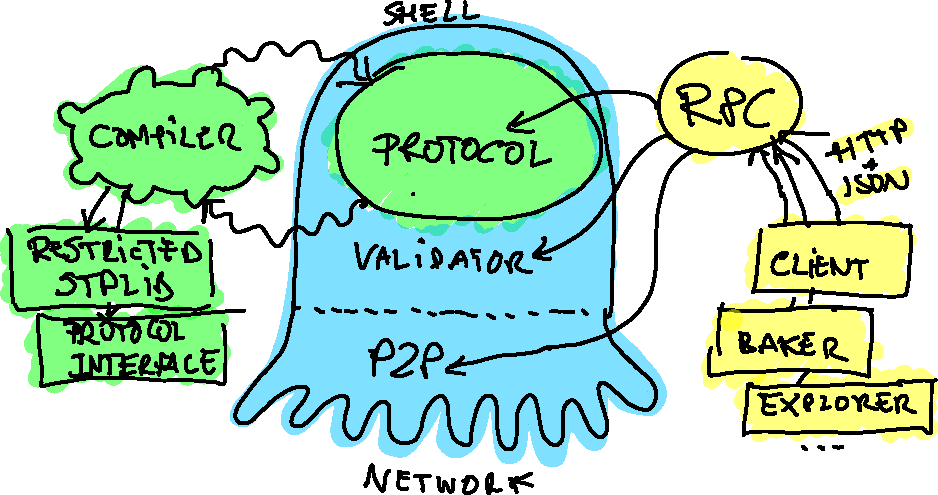
\includegraphics[width=\textwidth,keepaspectratio]{imagens/octupus.pdf}
    \caption{Architecture of Tezos (Source: Tezos Documentation)}
    \label{fig:octupus}

\end{figure}

In conclusion, the structure of Tezos is unique in that it separates the protocol, also known as the ``Economic Protocol'', from the rest of the node, called the shell. The protocol is responsible for interpreting transactions and administrative operations, while the shell includes the validator, peer-to-peer layer, disk storage of blocks, and versioned state of the ledger. The economic protocol on the chain is subject to amendment procedures, allowing for on-chain operations to switch from one protocol to another. The RPC layer allows clients, third-party applications, and daemons to interact with the node and its state. The communication between the shell and the protocol is based on the Updater.PROTOCOL interface, and the protocol is restricted to a specific environment to improve security. A Tezos node can contain multiple economic protocols, but only one of them is activated at any given time through a two-step activation process.


\subsection*{\textbf{Implementation of a Protocol}}

Implementing a Proof of Work consensus algorithm as a protocol for Tezos was motivated by several reasons. Firstly, it was an opportunity for hands-on learning about how protocols are implemented and structured. This understanding is crucial for later work, such as testing and adding an adaptive layer to the DSL mentioned in previous sections. It also allowed for a deeper understanding of how Tezos handles protocols and how they are executed in the Tezos node.

The implementation of Proof of Work was also significant because it provides a contrast to Tezos' original Proof of Stake protocol. This demonstrated that Tezos can be used to implement other types of consensus algorithms, including those that are different from the original. The implementation of Proof of Work also has the whole the concept of mining, which is not present in the Proof of Stake protocol.

Additionally, implementing a protocol in Tezos is a big accomplishment. The fact that only a few people do so makes this achievement even more significant, especially considering that it's a different type of consensus. This demonstrates a deep understanding of consensus algorithms and the ability to put that knowledge into practice.

In conclusion, the implementation of Proof of Work as a protocol for Tezos was a valuable learning experience that allowed for a deeper understanding of how protocols are structured and executed in Tezos. It also reinforced the concept of consensus algorithms and demonstrated the ability to put that knowledge into practice by implementing a unique protocol in Tezos.


\subsection*{Requirements of a Protocol In Tezos}
In order to implement the experiment of a Proof of Work consensus algorithm for Tezos, a "lib\_protocol" module in the protocol folder had to be created, where this is the main entry to the protocol and is executed by the node as the new amendment/consensus protocol. This is the only part that has to be implemented in OCaml and has to be compiled to work with the node.

To do so, a ``TEZOS\_PROTOCOL'' file must be included in this module, that is used to specify the version of the environment that the protocol is to be compiled against, which in this case the version 6 was the one used, the hash of the protocol folder and the set of modules implemented in the folder. 

There's the possibility to implement a newer environment for the protocol to accommodate the protocol, yet, for this experiment, this wasn't necessary. 

Like said previously, the environment is an interface that provides a set of OCaml modules that the protocol can use, and the interface used to interact with the Tezos Shell.

The most important functions and types in that had to be implemented for environment ``v6'' were:

\begin{itemize}
    % TODO: , mudar isto para código, no nome das coisas
    \item \emph{block\_header\_data}: This is the protocol-specific part of the header.
    \item \emph{block\_header}: This is the combination of the protocol header and the shell header.
    \item \emph{operation\_data}: This is the protocol-specific part of an operation/transaction.
    \item \emph{operation}: This is the combination of the protocol operation part and the shell operation part.
    \item \emph{validation\_state}: This is the state of the validation of a block or operation, passed between functions.
    \item \emph{init}: This function is executed to prepare the chain to start executing the new protocol.
    \item \emph{begin\_application}: This function is used when validating a block received from the network.
    \item \emph{begin\_partial\_application}: This function is used when the shell receives a block more than one level ahead of the current head. 
    \item \emph{begin\_construction}: This function is used by the shell when instructed to build a block and for validating operations as they are gossiped on the network.
    \item \emph{apply\_operation}: This function is called after \emph{begin\_application} or \emph{begin\_construction} and before \emph{finalize\_block} for each operation in the block or in the mempool, respectively. It validates the operation and updates the intermediary state accordingly.
    \item \emph{finalize\_block}: This function represents the last step in a block validation sequence.
\end{itemize}

In summary, the ``TEZOS\_PROTOCOL'' file is used to specify the protocol environment to be used by the Tezos node, and the environment provides a set of functions and types that the protocol must implement to be able to operate within the Tezos network.

\subsection*{Implementation of the module ``lib\_protocol''}

The implementation of a new protocol in the Tezos codebase is a significant challenge.
In this particular case, the goal was not only to implement the new protocol, but to also learn how existing protocols are structured and implemented within the Tezos codebase. The approach was to study and follow closely the implementation of existing protocols, rather than taking an easier approach that may also have resulted in a working protocol but would not have offered the same level of learning.

The protocol that was implemented includes a few functionalities, such as transactions between two entities, where ``Tez'', the currency used in Tezos, is transferred from one account to another.

Another aspect of the protocol is the concept of mining and verifying the proof of work, like mentioned in a previous section about Proof of Work.
This is done by hashing the header whole header, both the shell part and the protocol part, this last one containing the nonce, and verifying that the hash value is lower than the target where this is one of the main mechanism behind proof of work.

The environment that the protocol is compiled against requires a definition of the protocol header, which contains three elements: ``target'', ``nonce'', and ``miner''.

The \textbf{target} is used for comparison with the target value that the node calculated it should be (the specifics of how this is done is explained in a later point).
The \textbf{nonce} is used to achieve a header hash with a value lower than the target, which is a key part of the Proof of Work mechanism.
Finally, the \textbf{miner} field stores the address of the miner who found the nonce/hash, which is used to reward the miner. These elements combined make up the protocol-specific part of the header.


\subsection*{Implementation of Information Representation and Storage Logic}

The implementation of the protocol in Tezos involves defining and representing the various types of information that are necessary for the protocol to function. This includes things like accounts, constants, headers, time, target, currency (Tez), and operations.

The information stored in the protocol is abstracted, meaning that the protocol itself is stateless. The context in which the protocol is applied maps to the actual storage of the blockchain, but this is hidden from the protocol. The protocol only sees the storage as a generic key-value store and the functions that access this are defined in the "raw\_context.ml" file (in reality, they are accessed as a Tree, not just as a generic key-value). These functions allow the protocol to read, write, and update the storage, but the actual details of how this is done are not relevant to this document.


The Tezos Protocol is implemented through a series of files that represent various components and functionalities. In this section, we will take a closer look at the information stored and the logic behind each component in the protocol.

The protocol contains representations/definitions and operations of the following types/\\information, which are stored in files that end with ``repr.ml''. The Tezos documentation calls this the ``representation layer'' of the protocol.

\begin{itemize}

    \item Accounts/Manager: This represents the concept of an account in the protocol. An account is just a key, which is used to fetch information from the storage. It is a Public Key Hash.

    \item Constants/Parameters: This file contains information that is constant throughout the execution of the protocol. Some constants can be defined when activating the protocol. The constants include:

        \begin{itemize}
            \item \emph{block\_time}: Defines the time between blocks.
            \item \emph{initial\_target}: Defines the first target value.
            \item \emph{difficulty\_adjust\_epoch\_size}: Defines the number of blocks to wait to then readjust the target.
            \item \emph{halving\_epoch\_size}: Defines the number of blocks to wait to then halve the mining reward.
            \item \emph{reward\_multiplier}: The initial reward, which then gets halved.
            \item \emph{Header}: Defines the Protocol header, as mentioned before.
            \item \emph{block\_time}: Defines the time between blocks.
        \end{itemize}

    \item Time: Defines the type of time used throughout the protocol.

    \item Target: Defines how the target should be, in this case, it's a 256-bit number.

    \item Tez: Defines the type and operations for the currency.

    \item Operations: Representations and functionalities of the available operations. These include Transactions (between two entities) and Reveal (maps a Public Key to a Public Key Hash, like the ones used in the Accounts).

\end{itemize}

Some of these representations where designed by following the existing protocols implemented in the Tezos codebase. These representations ensure that the creation, conversion, encoding and decoding and other functionalities are done correctly by the protocol.

The logic behind storing information in the Tezos Protocol is an integral part of its functionality. The protocol uses an abstraction over the blockchain as its storage mechanism. 
The files that are responsible for storing information have names ending with ``-storage.ml'', and they store the following key pieces of information:
\begin{itemize}
    \item Accounts: It stores information about each account in the protocol. It maps the account's key to the account's balance and other important information and how defines how this information should be stored, retrieved and other checks.

    \item Target: It stores the current target, which is used for comparing the value of the header hash in the proof of work process.

    \item Epoch Time: It stores the timestamp of the latest difficulty adjust epoch, which is used to determine when it's time to adjust the target value. This is an important part of maintaining the security and integrity of the network, as it allows the network to dynamically adjust the difficulty of mining to ensure a stable rate of block production.
\end{itemize}

By storing these types of information in the blockchain, the Tezos Protocol provides a secure and transparent method of tracking the state of the network, which is crucial for the proper functioning of its operations. The protocol also provides a well-defined structure for the information it stores, which ensures consistency and maintainability of the code.

\subsection*{Implementation of the main entry points to the protocol}

The implementation of the main functions of the protocol plays a crucial role in ensuring the correct execution of the protocol. These functions are designed to take the necessary steps to apply the information and verify the validity of the information being applied. The functions presented in the previous section, such as \emph{begin\_application}, \emph{begin\_partial\_application}, etc. are all a part of the main functions of the protocol.

These functions perform various checks and updates to the context, which is an immutable representation of the state of the protocol. The context contains information such as the accounts, the target, and the epoch time, among others. The functions return some form of validation state and updated context, if applicable.

\begin{itemize}

    \item \emph{begin\_application} and \emph{begin\_partial\_application}:
        \begin{itemize}
            \item These functions prepare the current raw context, which contains information such as the context and more. The concept of raw context will be explained later.
            \item They perform checks, such as verifying if the current target is the correct one and if the header has a valid hash, that is, if the hash of the whole blockheader has a value lower than the target.
            \item They update information such as the target for the next epoch, if an epoch has elapsed.
        \end{itemize}

    \item \emph{begin\_construction}:
        \begin{itemize}
            \item Does the same preparation to the context as \emph{begin\_application} and \emph{begin\_partial\_application}.
            \item Performs the same checks, but also rewards the miner if the block is valid.
        \end{itemize}

    \item \emph{apply\_operation}:
        \begin{itemize}
            \item Verifies if the operation contains a valid signature.
            \item Verifies if the operation has a positive result, for example, if the account has enough funds to transfer to another account.
            \item If the operation is positive, it executes the operation on the current context.
        \end{itemize}

    \item \emph{finalize\_block}:
        \begin{itemize}
            \item Commits the change to the shell.
            \item Returns a receipt or result log that exposes what happened with the application of either a block or operation.
        \end{itemize}
    \item \emph{init:}
        \begin{itemize}
            \item Initializes everything needed to start the protocol, such as the constants and storage.
            \item Also creates the first blocked of the protocol to be appended to the chain.
        \end{itemize}
    \end{itemize}

The extensive logic involved in these functions will not be presented in this document, but it is important to understand the role they play in ensuring the correct execution of the protocol.


\subsection*{Implementation of Alpha and Raw Contexts}

The implementation of the protocol relies heavily on two core abstractions: \textbf{Alpha\_context} and \textbf{Raw\_context}. These two modules play crucial roles in ensuring the separation of concerns and allowing the protocol to be implemented over a generic key-value store.

Alpha\_context, defined in the ``alpha\_context.ml'' module, serves as the consensus view of the context. This module enforces the separation between mapping the abstract state of the ledger to the concrete structure of the key-value store, and implementing the protocol over the state. The Alpha\_context defines a type ``t'' that represents the abstracted state of the ledger and can only be manipulated through the use of selected manipulations, which preserve the well-typed aspect and internal consistency invariants of the state.

The abstracted state is read from the disk during the validation of a block and is updated by high-level operations that preserve consistency. Finally, the low-level state is extracted to be committed to disk. This abstraction provides a well-separated structure in the code, with the code below Alpha\_context handling the ledger’s state storage, and the code on top of it implementing the protocol algorithm using plain OCaml values.

Raw\_context, defined in the ``raw\_context.ml'' module, is the information view used by Alpha\_context. It serves as the raw, storage, or non-abstract view of what is actually done in the background by the consensus/protocol. Raw\_context provides the abstraction used by Alpha\_context to access the raw part of the protocol, that is, the information that is actually stored and the representation layer.

In conclusion, the implementation of the protocol relies heavily on Alpha\_context and Raw\_context to enforce separation of concerns and to abstract away the underlying implementation details, allowing the protocol to be implemented over a generic key-value store in a readable and well-separated manner.

\subsection*{Features that weren't implemented}
In this feasibility study, we have focused on the implementation of consensus protocol in the Tezos node. However, there are a few features that have not been included in this study but could be considered as future work.

One of the missing features is the support for smart contracts. This was not the main focus of the experiment, but smart contracts can be added on top of the protocol to provide more functionality. Currently, the protocol only supports peer-to-peer value transactions, but with the addition of smart contracts, more complex operations can be performed.

Another missing feature is the lack of upgradability in the protocol. This was intentional as this experiment was focused on a standalone Proof of Work consensus algorithm, and there is no previous protocol nor will there ever be a next protocol that is an amendment to this one. Upgradability could be added to the protocol in the future to provide more flexible and dynamic updates, but once again, for this kind of experiment, doing so would be useless.

It should be noted that the absence of these features was not due to technical limitations, but rather a deliberate decision to focus on the implementation of a protocol in the Tezos.

\subsection*{Tools developed to interact with the protocol}

In this study, tools related to the protocol were also implemented to enable interaction with the network. These tools could be developed independently from the Tezos project, since it's possible to communicate with the tezos node through JSON RPC. However, implementing these tools using OCaml and Tezos modules has the added benefit of being automatically integrated with the Tezos node client (and much more). Upon activation of the protocol, the client would automatically adapt to accommodate it, enabling commands that are specific to the protocol, such as ``Transfer'' and ``Reveal'', which is the case of the protocol covered here.

One of the tools implemented was the client, which can be found in the ``lib\_client'' folder. The client is mostly used to access information on the network, such as an account's balance or the current target. It serves as a better user interface for accessing the information through JSON RPC services. The client also has the capability of injecting blocks and operations into the network, so it can perform the two operations included in the protocol.

Another tool that was implemented is the baker, which can be found in the "lib\_baker" folder. The baker uses functionalities implemented in both the client module and the "Shell Services" module, this last one being already part of the Tezos codebase.
The baker performs the task of baking (how block creation is called in Tezos), or mining, a block by taking multiple operations, pre-applying the block in the protocol (to check if the block header is valid), and then performing the work to find the nonce that makes the block's hash lower than the target, similar to what a miner would do in a Proof of Work blockchain. Once the block is mined, it is pushed to the chain (and spread to the network).\\


In conclusion, this experiment proved to be a valuable exercise as it allowed us to gain a deeper understanding of how consensus protocols work and how they can be implemented within a blockchain network. The implementation of the protocol allowed us to test its capabilities, limitations and to identify areas for improvement. Furthermore, it demonstrated the versatility and flexibility of the Tezos network in accommodating custom consensus protocols, making it an ideal platform for experimentation and innovation.

\section{Future Tasks}

The research plan outlined below highlights the tasks that we intend to undertake in this thesis project. However, it should be noted that the direction of the project may evolve and change as we progress, leading to potential modifications to the plan. Nonetheless, this serves as a starting point for our research journey.

\textbf{Task 1}: Implementation of the Proof of Work (experiment) protocol in Tezos. The goal of this task is to implement a Proof of Work protocol in the Tezos blockchain, which is a well-known platform for experimenting with new consensus algorithms. This task is almost finished (as of the writing of the document).

\textbf{Task 2}: Testing of the Proof of Work protocol. In this task, we will test the Proof of Work protocol that was implemented in the previous task, to ensure that it is functioning correctly. This will also serve as another experiment to learn how to test this kind of algorithms in this environment.

\textbf{Task 3}: Development of a generic framework for adding new consensus algorithms. The aim of this task is to make it easier and more straightforward to add new consensus algorithms to the Tezos platform. This will be achieved by developing a generic framework that can be easily adapted to support new protocols.

\textbf{Task 4}: Creation of a platform for testing consensus algorithms in case there are limitations with Tezos. In this task, we will create a platform that will allow us to test various consensus algorithms, including the Proof of Work protocol that was implemented in task 1. This platform will be used to compare the performance and efficiency of different protocols. Tezos already has fine-tunning and testing platform, but a new one will be developed in the event that limitations arise with the use of Tezos'.

\textbf{Task 5}: Integration of a Domain-Specific Language (DSL) for consensus algorithms. The goal of this task is to make it easier to integrate new consensus algorithms into the Tezos platform, by using the Lupin DSL (\ref{lupin}) that can be adapted to support different protocols. The knowledge gained from the development of the generic framework for adding new consensus algorithms in task 3 will be used as input for this task.

\textbf{Task 6}: Development of additional tools for blockchain consensus algorithms. In this task, we will continue to build on the knowledge gained from the previous tasks, and develop additional tools that can be used to improve the performance and efficiency of blockchain consensus algorithms.

\textbf{Task 7}: Writing of the thesis. The thesis will present the research results and provide conclusions based on the work performed in the previous tasks. The writing of the thesis will be a final step, but will be done concurrently with the other tasks.

In addition to these tasks, we may consider incorporating additional features or making improvements to existing features, depending on the results of our research and the progress of our work. The aim is to continue advancing the state of the art in the field of blockchain consensus algorithms, and to provide a comprehensive understanding of the various protocols and tools that are available for improving the performance and efficiency of blockchain networks.


\section{Conclusion}

In conclusion, this project has explored the crucial concepts of in the field of blockchain technology. Through a review of the state of the art, it was revealed that there are several popular consensus algorithms used in blockchain networks, each with its own strengths and weaknesses. The project then identified the challenges in the field of consensus protocols, including the lack of standardization, difficulties in comparison, testing and the fact that there's a multitude of different consensus algorithms available in the field of blockchain technology,
making it difficult for individuals and organizations to adopt blockchain effectively.

The proposed solution was to overcome these challenges by providing a method of testing and easily swapping consensus algorithms in a pre-existing well-tested blockchain network.
The implementation of this solution was tested and proved to be feasible by the execution of the experiment done, demonstrating the versatility and flexibility of the Tezos network in accommodating custom consensus protocols.

The document also outlined the main contributions, goals, and objectives for future work.
The next phase of the project will focus on the completion and testing of the Proof of Work (experiment) protocol implemented in Tezos, development of a generic framework for adding new consensus algorithms, creation of a platform for testing them, integration with the Lupin DSL, and writing of the thesis to present research results and conclusions on the work performed. The aim is to advance the state of the art in blockchain consensus algorithms and provide a comprehensive understanding of available protocols and tools to improve block\-chain network performance and efficiency.





\end{comment}
\chapter{Conclusion}

In conclusion, this project has explored the crucial concepts of eBPF-based security. Through a review of the state of the art, it was made clear that although several tools leverage eBPF for security purposes, none of those have gone through the process of formal verification. 

The proposed solution is to develop an eBPF based tool, and submit it to the process of rigorous testing and formal verification, as to guarantee the safety and correctness of said tool. The experiment presented is to be seen as a first step in achieving this goal. 

The document also outlined the main contributions, goals, and objectives for future work. 
The next phase of the project will focus on the completion and testing of the target eBPF application, the formal verification process of it, leaving open the possibility of additional features and targets to be presented along the way. The aim is to advance the state of the art in the security field, specifically on data exfiltration prevention.






%% Fim da inserção dos capitulos


%% Inicio Bibliografia
\cleardoublepage
\phantomsection
\addcontentsline{toc}{chapter}{Bibliografy}
%%%%%%%%%%%%%%%%
% Escolher entre as duas opcções
%
% A primeira é uma forma livre
% A segunda é a utilizada pelo IEEE
%
%Primeira opcção
%\bibliographystyle{estilo-biblio}				%Estilo bibliografia com nomes
%\bibliography{bibliografia}					%Entrada biblbiografia aconselhada com nomes
%
% Segunda opcção
\bibliographystyle{IEEEtran}					%Estilo bibliografia IEEE
\bibliography{IEEEabrv,bibliografia}				%Entrada bibliografia aconselhada para IEEE
%% Fim Bibliografia


%%Anexos
%\appendix
 
%\chapter{Anexos}
\label{chap:anexos}

\section{Datasheets dos componentes utilizados}


%\cleardoublepage


%%Glossário
%\newpage
%\section*{\titulos{Glossário}}
%\vspace{0.5cm}
%	\noindent\begin{tabularx}{\linewidth}{l p{0.5cm} Y}
%	\LaTeX & & Conjunto de macros para o processador de textos \TeX, utilizado amplamente para a produção de textos matemáticos e científicos devido à sua alta qualidade tipográfica.\cr
%	\end{tabularx}
%\cleardoublepage



%%Inserir índice remissivo
%\printindex

\end{document}
